\documentclass[10pt,pdf,hyperref={unicode}]{beamer}

\usepackage[utf8]{inputenc}
\usepackage[russian]{babel}
\usepackage{amssymb,amsmath}
\textwidth=10.7cm % ширина текста


\usepackage{color}
\usepackage{url}

\usepackage{indentfirst}
\usepackage{graphicx}

\usetheme{Warsaw}%Goettingen}


\title{Построение ансамбля алгоритмов рекомендаций}
\subtitle{Выпускная квалификационная работа}

%\author{Кудрявцев Георгий}
\institute{\begin{flushright}
      \parbox{0.5\textwidth}{
        \raggedleft
        \textbf{Выполнил:}\\
        студент 417 группы\\
        Кудрявцев Георгий Алексеевич\\[5mm]
        \textbf{Научный руководитель:}\\
        д.ф-м.н., профессор\\
        Дьяконов Александр Геннадьевич
      }
    \end{flushright}}
\date{\today}
\begin{document}
\frame{\titlepage}
%\AtBeginSection{
%    \begin{frame}
%        \frametitle{Содержание}
%        \tableofcontents[currentsection]
%        \end{frame}
%}

\begin{frame}{Неформальная постановка задачи}
Требуется улучшить качество работы алгоритмов ранжирования при помощи ансамблирования уже существующих методов.
\end{frame}

\begin{frame}{Предметная область}
 Рассматривается задачи ранжирования по данным с двоичной релевантностью.
 
 На практике данная задача решается при помощи алгоритмов машинного обучения.
 
 В данной работе рассматриваются факторизационные методы и их линейные ансамбли.
\end{frame} 

\begin{frame}{Актуальность задачи}

Построение рекоммендаций для:

\begin{itemize}
\item социальных сетей

\item сайтов знакомств

\item интернет магазинов
\end{itemize}
\end{frame}

\begin{frame}{Цель и задачи}
Цель: разработать метод ансамблирования, который стабильно улучшает качество ранжирования.

Задачи: 

\begin{itemize}
\item Составить обзор современных факторизационных методов ранжирования. 

\item Предложить эффективный метод ансамблирования.

\item Реализовать методы и провести их сравнительный анализ.

\end{itemize}
\end{frame}

\begin{frame}{Формальная постановка задачи}

\textbf{Входные данные}:

 матрица $R$ размера $M \times N$, где $M$ - количество пользователей, $N$ - количество предметов. $R_{ui}$ = 1, если пользователей $u$ взаимодействовал с предметов $i$. В противном случае $R_{ui}$ = 0.

\textbf{Выходные данные}: 

Для каждого пользователя $u$ ранжированный список предметов, которые не лежат в тренировочной выборке.
\end{frame}

\begin{frame}{Обзор существующих методов}

\begin{itemize}
\item \textbf{CLiMF}\footnote{Yue Shi, Alexandros Karatzoglou, Linas Baltrunas.
CLiMF: learning to maximize reciprocal rank with collaborative less-is-more filtering. 2012}
 -- Факторизационный метод, который оптимизирует сглаженную версию метрики MRR.
  	
\item \textbf{MPR\_MF}\footnote{Steffen Rendle, Christoph Freudenthaler, Zeno Gantner.    
         BPR: Bayesian Personalized Ranking from Implicit Feedback. 2009}
-- Факторизационный метод, который оптимизирует AUC.
\item \textbf{TFMAP}\footnote{Yue Shia,Alexandros Karatzogloub, Linas Baltrunas.
TFMAP: Optimizing MAP for Top-N Context-aware Recommendation. 2012} 
-- Факторизационный метод, который оптимизирует сглаженную метрику MAP.
\item \textbf{iMF}\footnote{Yifan Hu, Yehuda Koren, Chris Volinsky.
	Collaborative Filtering for Implicit Feedback Datasets. 2008}
-- Факторизационный метод, который оптимизирует взвешенную квадратичную ошибку.
\end{itemize}
\end{frame}

\begin{frame}{Линейный ансамбль}
Пусть имеется множество базовых алгоритмов $b_i(x)$. 

Необходимо подобрать такие веса $\alpha_i$, чтобы линейная комбинация алгоритмов $\hat{b}(x) = \sum_i \alpha_i b_i(x)$ показывала лучший результат по какому-нибудь заданному функционалу. 
\end{frame}

\begin{frame}{Оптимальное взвешенное голосование}

 Рассмотрим линейную комбинацию двух алгоритмов ранжирования  в следующем виде:
\begin{equation*}
	\hat{f}_{ui} = \alpha f_{ui}^{m_1} + (1 - \alpha) f_{ui} ^ {m_2} \textrm{\ , где $0 \leq \alpha \leq 1$}
\end{equation*} 
	
\begin{figure}[h]
\center{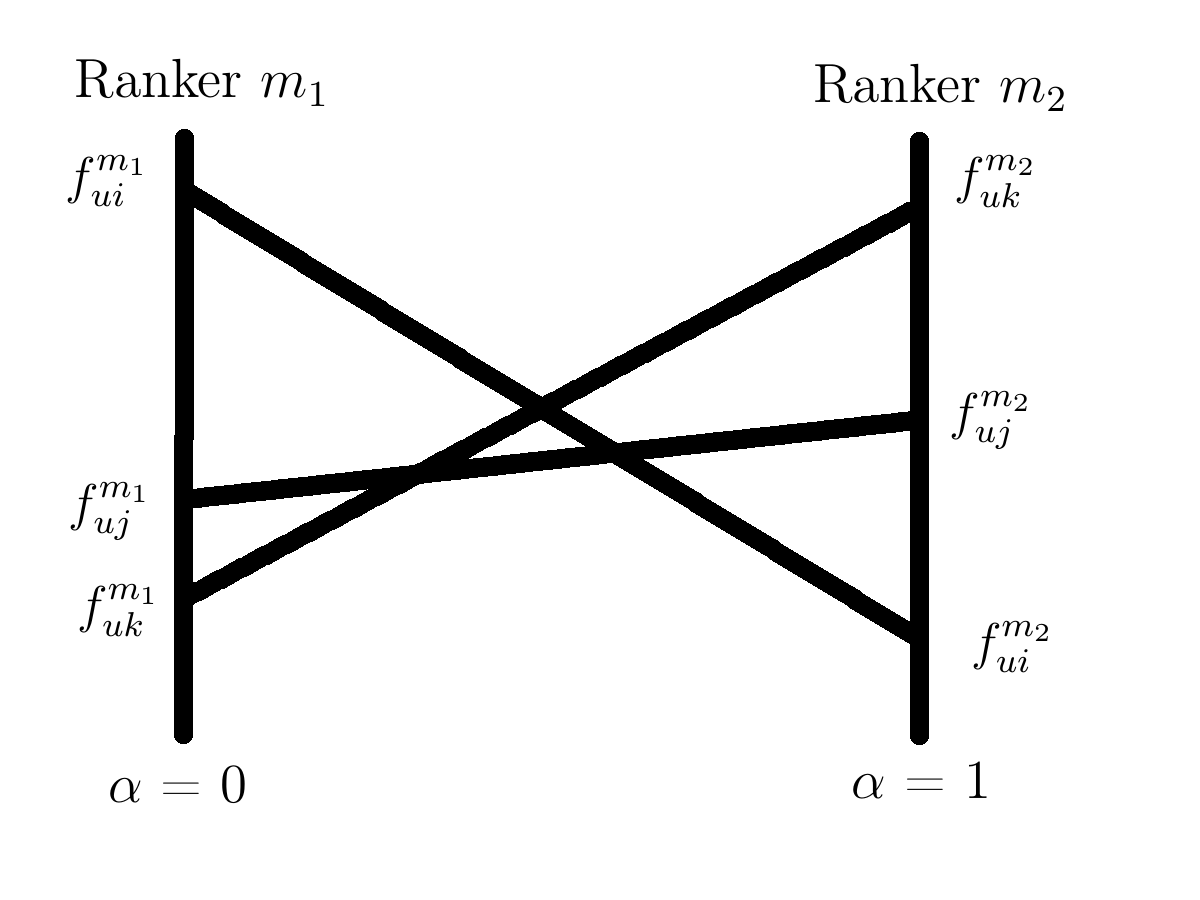
\includegraphics[width=0.4\linewidth]{latexpic}}
\caption{Графическая демонстрация идеи метода \footnote{Qiang Wu, Christopher J. C. Burges, Krysta M. Svore.	 Adapting Boosting for Information Retrieval Measures. 2010.}}
\label{pic:latexpic}
\end{figure}

\end{frame}

\begin{frame}{Экспериментальные оценка}

\begin{table}[H]
\begin{flushleft}
\resizebox{0.7\textwidth}{!}{\begin{minipage}{\textwidth}
\begin{tabular}{|c|c|c|c|c|c|c|c|c|c|c|}
\hline
 \multicolumn{11}{|c|}{MovieLens 100k} \\
\hline
& \multicolumn{5}{|c|}{ptest = 10\%, pvalid=10\%, maxiter = 5} & \multicolumn{5}{|c|}{ptest = 20\%, valid = 10\%, maxiter = 5}\\
\hline
  & BSM  & SV &  RV & OVB & OVT &BSM  & SV & RV & OVB & OVT \\
\hline
P@5 & 0.2965 & 0.1602 &	0.2528 & \textbf{0.3069} & 0.3019 & 0.4451 &	0.2531 & 0.3831 & \textbf{0.4498} & 0.4464 \\
\hline
1call@5 & 0.7344 & 0.4950 & 0.6712 & \textbf{0.7580} & 0.7555 & 0.8706 & 0.6203 & 0.8039 &	\textbf{0.8784} & 0.8734\\
\hline
NDCG@5 &0.3201 & 0.1778 & 0.2783 & \textbf{0.3307} &	0.3257 & 0.4705 & 0.2738 & 0.4070 &	\textbf{0.4770} & 0.4752\\
\hline
MAP@5 & 0.5035 & 0.3239 & 0.4599 & \textbf{0.5185} & 0.5152 & 0.6480 & 0.4261 & 0.5763 &	0.6555 & \textbf{0.6562}\\
\hline
 \multicolumn{11}{|c|}{Epinion} \\
\hline
& \multicolumn{5}{|c|}{ptest = 10\%, pvalid=10\%, maxiter = 5} & \multicolumn{5}{|c|}{ptest = 20\%, valid = 10\%, maxiter = 5}\\
\hline
  & BSM  & SV &  RV & OVB & OVT &BSM  & SV & RV & OVB & OVT \\
\hline
P@5 & 0.0716 & 0.0295 &	0.0534 & \textbf{0.0764} & 0.0760 & 0.1283 &	0.0550 & 0.1000 & 0.1328 & \textbf{0.1363} \\
\hline
1call@5 &0.2710 & 0.1303 & 0.2183 &	\textbf{0.2921} & 0.2908 & 0.4179 & 0.2242 &	0.3595 & 0.4372 & \textbf{0.4438}\\
\hline
NDCG@5 &0.0775  & 0.0334 & 0.0572 &	\textbf{0.0830} & 0.0822 &  0.1384 &	0.0615 & 0.1062 & 0.1425 &	\textbf{0.1468}\\
\hline
MAP@5 & 0.1561 & 0.0759 & 0.1193 & \textbf{0.1688} & 0.1672 & 0.2536 & 0.1316 & 0.2035 & 0.2607 & \textbf{0.2686}\\
\hline
\end{tabular}
\end{minipage}}
\end{flushleft}
\end{table}

\end{frame}

\begin{frame}{Экспериментальные оценка}

\begin{table}[H]
\begin{flushleft}
\resizebox{0.7\textwidth}{!}{\begin{minipage}{\textwidth}
\begin{tabular}{|c|c|c|c|c|c|c|c|c|c|c|}
\hline
 \multicolumn{11}{|c|}{Slashdot} \\
\hline
& \multicolumn{5}{|c|}{ptest = 10\%, pvalid=10\%, maxiter = 5} & \multicolumn{5}{|c|}{ptest = 20\%, valid = 10\%, maxiter = 5}\\
\hline
  & BSM  & SV &  RV & OVB & OVT &BSM  & SV & RV & OVB & OVT \\
\hline
P@5 & 0.0431 & 0.0186 &	0.0291 & \textbf{0.0438} & 0.0436 &  0.0746 & 0.0362 & 0.0519 &	0.0757 & \textbf{0.0758}\\
\hline
1call@5 & 0.1644 & 0.0866 & 0.1272 & \textbf{0.1683} & 0.1671 & 0.2570 & 0.1577 & 0.2038 & 0.2631 & \textbf{0.2653} \\
\hline
NDCG@5 & 0.0473 & 0.0201 &	0.0312 & \textbf{0.0481} & \textbf{0.0481} & 0.0803 &	0.0397 & 0.0556 & 0.0819 & \textbf{0.0822}\\
\hline
MAP@5 & 0.0959 & 0.0455 & 0.0684 & 0.0976 & \textbf{0.0978} & 0.1506 & 0.0877 & 0.1140 & 0.1550 & \textbf{0.1562}\\
\hline
 \multicolumn{11}{|c|}{Movie Lens 1m} \\
\hline
& \multicolumn{5}{|c|}{ptest = 10\%, pvalid=10\%, maxiter = 5} & \multicolumn{5}{|c|}{ptest = 20\%, valid = 10\%, maxiter = 5}\\
\hline
  & BSM  & SV &  RV & OVB & OVT &BSM  & SV & RV & OVB & OVT \\
\hline
P@5 & 0.2601 & 0.1065 &	0.2374 & 0.2628 & \textbf{0.2639} &  0.3936 & 0.1974 & 0.3616 &	\textbf{0.3983} & 0.3944\\
\hline
1call@5 & 0.6541 & 0.3424 & 0.6186 & 0.6566 & \textbf{0.6593} & 0.7985 & 0.5255 & 0.7714 & \textbf{0.8075} & 0.8066\\
\hline
NDCG@5 & 0.2795 & 0.1104 & 0.2476 &	0.2830 & \textbf{0.2836} & 0.4127 &	0.2007 & 0.3710 & \textbf{0.4192} & 0.4157\\
\hline
MAP@5 & 0.4384& 0.1936 & 0.3859 & 0.4440 & \textbf{0.4438} & 0.5729 & 0.3127 & 0.5166 & \textbf{0.5839} & 0.5822\\
\hline

\end{tabular}
\end{minipage}}
\end{flushleft}
\end{table}

\end{frame}

\begin{frame}{Результаты работы}

\begin{enumerate}

\item Составлен обзор основных факторизационных методов для задачи ранжирования для набора данных с двоичной релевантностью.

\item Предложен метод ансамблирования, который стабильной улучшает качество работы ранжирования.

\item Реализованы факторизационные методы  и эксперименты на языке python и c++.
\end{enumerate}

\end{frame}


\end{document}





